\documentclass[12pt]{article}

\usepackage{graphicx} % Required for including images
\usepackage{booktabs} % For professional looking tables
\usepackage[margin=1in]{geometry} % Set margins
\usepackage{hyperref} % For hyperlinks
\usepackage{float} % For image placement


\title{Performance Assessment of CPU and Disk Components Using Discrete-Time Event Simulation}
\author{Evan Smtih\\
        CS4328 Operating Systems\\
        Mina Guirguis, Ph.D.\\}
\date{\today}

\begin{document}

\maketitle

\section{Abstract}
This report presents the findings from a series of experiments conducted to assess the performance of CPU and Disk components of an operating system under varying workloads using a discrete-time event simulator. The objective was to understand how different rates of process arrivals (denoted by lambda, $\lambda$) affect key system performance metrics.

\section{Running the Simulator}
The simulation can be executed directly from the command line by providing specific arguments related to the simulation's configuration. Follow these steps to run the simulator:

\begin{enumerate}
    \small\item Open your terminal or command prompt.
    \small\item Navigate to the directory where the simulation scripts are located.
    \small\item Download the get-pip script using curl:
    \begin{verbatim}
[user]$ curl https://bootstrap.pypa.io/get-pip.py -o get-pip.py
    \end{verbatim}
    \small\item Run the get-pip script:
    \begin{verbatim}
[user]$ python get-pip.py
    \end{verbatim}
    \small\item Install the required dependencies using the following command:
    \begin{verbatim}
[user]$ python -m pip install matplotlib pandas
    \end{verbatim}
    \small\item Run the simulation using the following command format:
    \begin{verbatim}
[user]$ python main.py <lambda> <average_CPU_service_time> <average_Disk_service_time>
    \end{verbatim}
\end{enumerate}

\section{Introduction}
The discrete-time event simulation project aims to evaluate the performance of two critical operating system components: the CPU and Disk. By simulating different workload intensities, this study provides insights into the system's behavior under various conditions.

\section{Methodology}
The simulator was designed to model the process flow within an operating system, focusing on the interaction between processes and the CPU/Disk components. Processes arrive at an average rate following a Poisson distribution, and service times are exponentially distributed.

\section{Implementation Details}
The simulation is structured around several key classes: CPU, Disk, Process, Event, and Simulator. These components work together to mimic the scheduling and processing of tasks within an operating system environment.

\section{Results}
This section presents the simulation results, showing how system performance metrics vary with different process arrival rates ($\lambda$).

\subsection{Average Turnaround Time}
\begin{figure}[H]
\centerline{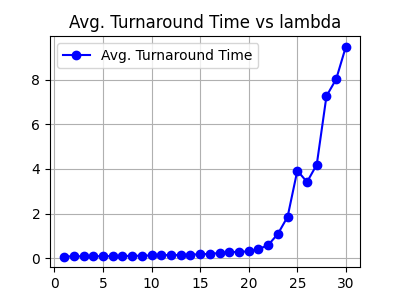
\includegraphics{figs/Avg. Turnaround Time_vs_lambda.png}}
\caption{Average Turnaround Time vs. $\lambda$}
\end{figure}

\subsection{Average Throughput}
\begin{figure}[H]
\centering
\centerline{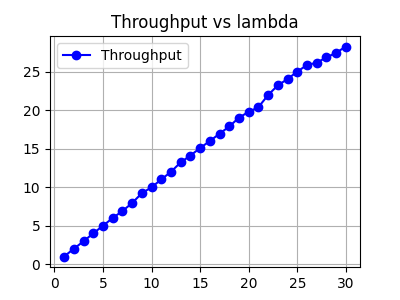
\includegraphics{figs/Throughput_vs_lambda.png}}
\caption{Average Throughput vs. $\lambda$}
\end{figure}

\subsection{CPU Utilization}
\begin{figure}[H]
\centering
\centerline{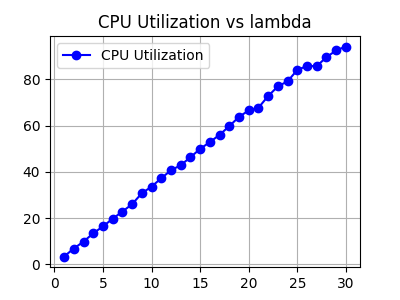
\includegraphics{figs/CPU Utilization_vs_lambda.png}}
\caption{CPU Utilization vs. $\lambda$}
\end{figure}

\subsection{Disk Utilization}
\begin{figure}[H]
\centering
\centerline{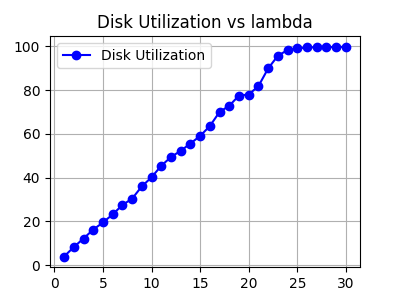
\includegraphics{figs/Disk Utilization_vs_lambda.png}}
\caption{Disk Utilization vs. $\lambda$}
\end{figure}

\subsection{Average Number of Processes in Ready Queue}
\begin{figure}[H]
\centering
\centerline{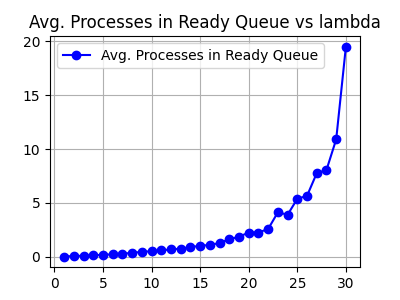
\includegraphics{figs/Avg. Processes in Ready Queue_vs_lambda.png}}
\caption{Average Processes in Ready Queue vs. $\lambda$}
\end{figure}

\subsection{Average Number of Processes in Disk Queue}
\begin{figure}[H]
\centering
\centerline{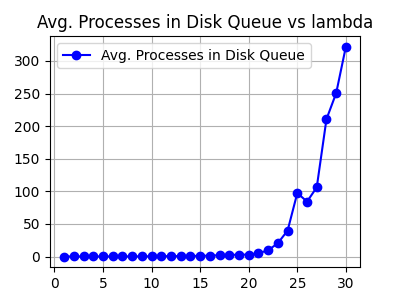
\includegraphics{figs/Avg. Processes in Disk Queue_vs_lambda.png}}
\caption{Average Processes in Disk Queue vs. $\lambda$}
\end{figure}

\section{Analysis}
The plots reveal a direct relationship between the process arrival rate and system performance metrics. As $\lambda$ increases, both the average turnaround time and system utilization rates exhibit noticeable trends, indicative of the system's capacity and efficiency in processing tasks.

\section{Conclusion}
The discrete-time event simulation project has successfully demonstrated the impact of varying workload intensities on the performance of CPU and Disk components. These findings provide valuable insights into the design and management of operating systems to ensure optimal performance under different conditions.

\end{document}
